% Created 2016-02-26 Fri 16:44
% Intended LaTeX compiler: pdflatex
\documentclass[11pt]{article}
\usepackage[utf8]{inputenc}
\usepackage[T1]{fontenc}
\usepackage{graphicx}
\usepackage{grffile}
\usepackage{longtable}
\usepackage{wrapfig}
\usepackage{rotating}
\usepackage[normalem]{ulem}
\usepackage{amsmath}
\usepackage{textcomp}
\usepackage{amssymb}
\usepackage{capt-of}
\usepackage{hyperref}
\usepackage{minted}
\usepackage[margin=0.5in]{geometry}
\usepackage{amsmath}
\usepackage{amsfonts}
\newcommand{\Problem}[1]{\subsection*{Problem #1}}
\newcommand{\Q}[1]{\subsubsection*{Q.#1}}
\newcommand{\union}[1]{\underset{#1}{\cup} }
\newcommand{\bigunion}[1]{\underset{#1}{\bigcup} \, }
\newcommand{\inter}[1]{\underset{#1}{\cap} }
\newcommand{\biginter}[1]{\underset{#1}{\bigcap} }
\newcommand{\minimize}[3]{\optimize{#1}{#2}{#3}{min}}
\newcommand{\maximize}[3]{\optimize{#1}{#2}{#3}{max}}
\DeclareMathOperator{\cov}{cov}
\DeclareMathOperator{\var}{var}
\author{Bachir El khadir}
\date{\textit{<2016-02-23 Tue>}}
\title{Problem set 2, ORF523}
\hypersetup{
 pdfauthor={Bachir El khadir},
 pdftitle={Problem set 2, ORF523},
 pdfkeywords={},
 pdfsubject={},
 pdfcreator={Emacs 24.5.1 (Org mode )}, 
 pdflang={English}}
\begin{document}

\maketitle



\section{Problem 1}
\label{sec:orgheadline1}
\begin{enumerate}
\item Let's consider a polynomial of degree 2: \(P(x) = x^TQx + bx + c\), \(P(x)\) can also be written as \(\frac12 x^T(Q + Q^T)x + bx + c\), so we can assume without loss of generality that \(Q\) is symmetric.

If \(Q\) is symmetric, by the eigen value decomposition theorem there exist \(U\) an orthogonal matrix and \(\Lambda\) a diagonal matrix such that \(Q = U\Lambda U^T\).

Let's denote \(\Lambda^+ = max(\Lambda, 0)\), \(\Lambda^- = min(-\Lambda, 0)\), then: \(Q = \underbrace{U\Lambda^+ U^T}_{S^+} -  \underbrace{U\Lambda^- U^T}_{S^-}\).

We have that \(\frac12 x^TS^+x + bx + c\) and \(\frac12 x^TS^-x\) are both convexe because their hessians (\(S^+\) and \(S^-\) respectively) is non-negative.
\item \begin{minted}[frame=lines,linenos=true]{matlab}
syms x y z;
f = (x^2 + 9/4* y^2 + z^2 - 1)^3 - x^2 * z^3 - 9/80*y^2 * z^3;
tf = simplify(taylor(f, [x, y, z], [0, 1/2, 1/2], 'Order', 3));
ans=char(tf)
\end{minted}
\end{enumerate}

\begin{align*}
P(x, y, z) &= -\frac{5}{256} x^2 - \frac{13437}{5120}y^2 - \frac{639}{1280}z^2 - \frac{837}{320}yz
+ \frac{5319}{1280} y + \frac{2421}{1280} z  - \frac{16371}{10240}\\
&= -a x^2 - b y^2 - c z^2 - d yz + e y + fz - h
\\&=  \underbrace{(f + \frac{d^2}{4b}) z^2}_{\text{convexe}}  - \underbrace{(a x^2 - e y - fz + h + b(y + \frac{d}{2b}z)^2)}_{\text{convexe}} 
\end{align*}

With numbers:

$$P(x, y, z) = \frac{2862801}{32000} z^2 - (\frac{5}{256} x^2 - \frac{5319}{1280} y - \frac{2421}{1280} z + \frac{16371}{10240} + \frac{13437}{5120}(y + \frac{1674}{25}z)^2)$$


\section{Problem 2}
\label{sec:orgheadline3}

The constraints \(A_1+A_2+A_3 \le 2 \max(0, T_1+T_2+T_3 - 3)\) leads to \(A_1 = A_2 = A_3\), eg \(T_1 + T_2 + T_3 = 3 = b\).
The next constraints \(A_1 + A_2 + A_3 + \ldots  + A_i \le 2\max(0, T_1 + T_2 + T_3 + \ldots + T_i- 3)\) can be written equivalently as : \(A_4 + \ldots + A_i \le 2(T_4 + \ldots + T_i)\) for \(i > 3\)


Let \(N = 24\)
Let \(\gamma_i := \theta(\alpha T_i + \beta A_i)\), then \(s_i = (1-\theta)s_{i-1} + \gamma_i\), by immediate induction \(s_i = \sum_{j=1}^i (1-\theta)^{i-j} \gamma_j\),
and

\begin{align*}S &= \sum_{i=1}^{N} \sum_{j \le i} (1-\theta)^{i-j} \gamma_j
\\&= \sum_{j=1}^N \gamma_j (\sum_{i=j}^N(1-\theta)^{i-j})
\\&= \sum_{j=1}^N \gamma_j \frac{1 - (1-\theta)^{N-j+1}}{\theta} 
\\&= \sum_{j=1}^N (\alpha T_i + \beta A_i) (1 - (1-\theta)^{N-j+1})
\\&= \langle \Theta, \alpha T + \beta A \rangle
\end{align*}

Where \(\Theta_i = (1 - (1-\theta)^{N-i+1})\)

We denote by \(X^{(k)}\) a quantity \(X\) that relates to the group \(k\), therefore \(CES^{(k)} = \langle \Theta^{(k)}, \alpha^{(k)} T + \beta^{(k)} A \rangle\) for \(k = 1, 2, 3\)

Optmizing the individual CES:
  \begin{align}
  \text{maximize} \; & \langle \Theta^{(k)}, \alpha^{(k)} T + \beta^{(k)} A \rangle \\
  \text{subject to} \; & A + T = 1,
    \\& A, T \ge 0
    \\& \sum_4^i A_j \le  2 \sum_4^i T_j \quad i = 4, \ldots, 24
\end{align}

\begin{minted}[frame=lines,linenos=true]{matlab}
%% Input
a = 2;
b = 3;
theta = [0.05 0.1 0.3];
alpha = [-0.1 0.8 -0.3];
beta = [1.4 -0.3 0.7];
num_periods = 24;
num_groups = 3;
Theta = zeros(num_groups, num_periods);

for k=1:num_groups
    for i=1:num_periods
        Theta(k, i) = 1 - (1-theta(k))^(num_periods-i+1);
    end
end

%% Results
table = zeros(num_groups+1, num_groups);
figures = []

%% Maximize individual CES
for group=1:3
    cvx_begin quiet
    variable T(num_periods);
    variable A(num_periods);
    maximize( Theta(group,:) * (alpha(group) * T + beta(group) * A))
    A + T == 1;
    0 <= T <= 1;
    0 <= A <= 1;
    T(1:b) == 1;
    for i = 4 : num_periods
        sum(A((b+1):i)) <= a* sum(T((b+1):i))
    end
    cvx_end

    figures(group) = figure('visible', 'off')
    subplot(2,1,1)
    title('s_i')
    % calculate s_i
    for k=1:3
        s = zeros(num_periods+1, 1);
        for i=2:(num_periods+1)
            s(i) = (1- theta(k)) * s(i-1) + theta(k) * (alpha(k) * T(i-1) ...
                                                        + beta(k) * (1-T(i-1)));
        end
        table(group, k) = sum(s);
        hold all
        plot(s(2:num_periods), '*-');
        legend(int2str(k));
    end
    legend('1', '2', '3')
    subplot(2,1,2);
    plot(round(T, 2), '*-');
    title('Theory proportion');
end
ans = table
\end{minted}



Maximizing the minimum of  all three CES at the same time
\begin{align}
  \text{maximize} \; & t \\
  \text{subject to} \; & A + T = 1,
  \\& A, T \ge 0
  \\& \sum_4^i A_j \le  2 \sum_4^i T_j \quad i = 4, \ldots, 24
  \\& t = \min_{k = 1, 2, 3} \langle \Theta^{(k)}, \alpha^{(k)} T + \beta^{(k)} A \rangle 
\end{align}


\begin{minted}[frame=lines,linenos=true]{matlab}
%% max min CES
cvx_begin
variable T(num_periods);
variable A(num_periods);
maximize( min(...
[Theta(1,:) * (alpha(1) * T + beta(1) * A);
Theta(2,:) * (alpha(2) * T + beta(2) * A);
Theta(3,:) * (alpha(3) * T + beta(3) * A)]))
A + T == 1;
0 <= T <= 1;
0 <= A <= 1;
T(1:b) == 1;
for i = 4 : num_periods
    sum(A((b+1):i)) <= a* sum(T((b+1):i))
end
cvx_end

figures(4) = figure('visible', 'off')

subplot(2,1,1)
title('s_i')
% calculate s_i
for k=1:3
    s = zeros(num_periods+1, 1);
    for i=2:(num_periods+1)
        s(i) = (1- theta(k)) * s(i-1) + theta(k) * (alpha(k) * T(i-1) ...
                                                    + beta(k) * (1-T(i-1)));
    end
    table(4, k) = sum(s);
    hold all
    plot(s(2:num_periods), '*-')
end
legend('1', '2', '3')
subplot(2,1,2);
plot(round(T, 2), '*-');
title('Theory proportion');
for p=1:4
    saveas(figures(p),[ 'img/plan' int2str(p)], 'png')
end

ans = table
\end{minted}


\begin{org}
\begin{table}[htb]
\caption{Table of CES for different groups / plans}
\centering
\begin{tabular}{lrrr}
plans & group 1 & group 2 & group 3\\
\hline
plan 1 & 7.4159 & 3.0522 & 5.9452\\
plan 2 & -1.0548 & 12.574 & -6.5001\\
plan 3 & 7.4159 & 3.0522 & 5.9452\\
plan 4 & 5.1884 & 4.9813 & 4.9813\\
\end{tabular}
\end{table}
\end{org}



\subsection{Figures}
\label{sec:orgheadline2}

\begin{center}
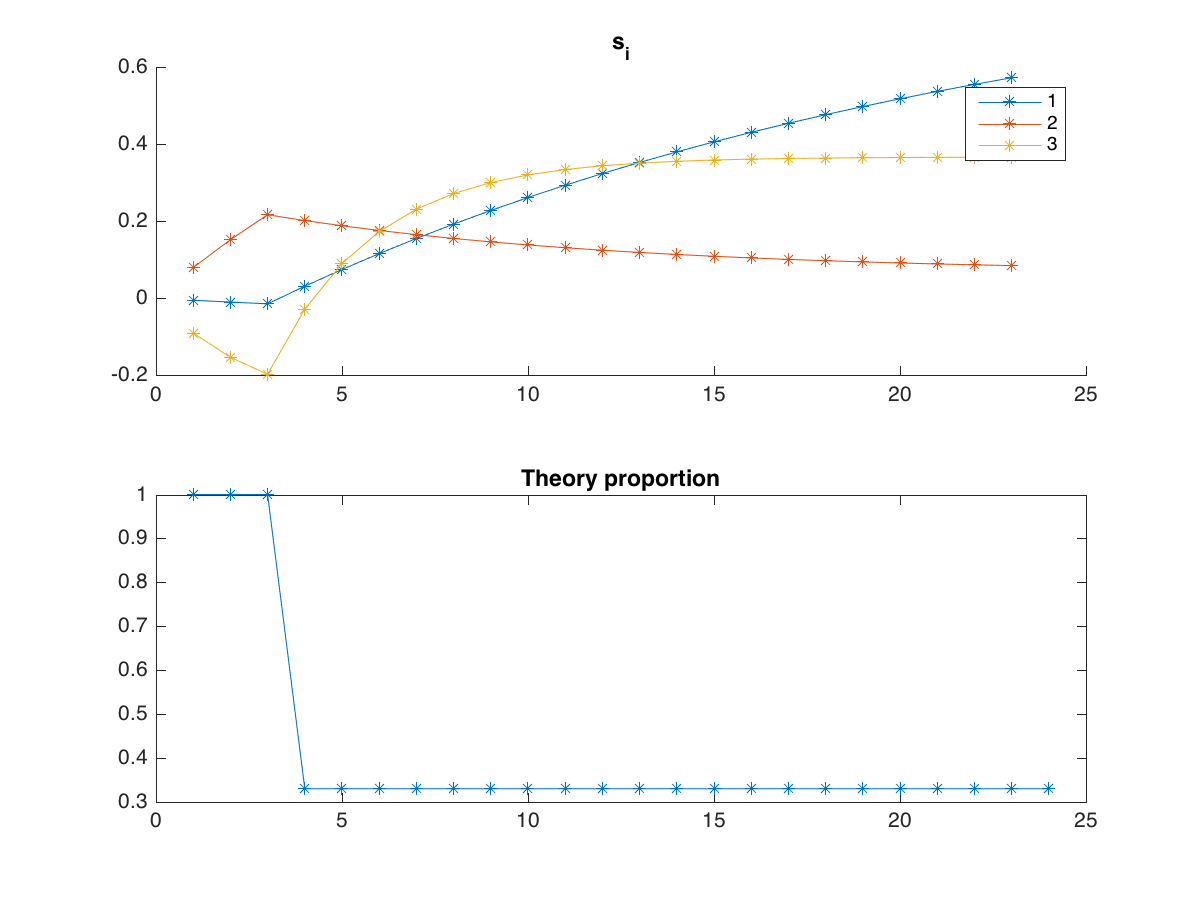
\includegraphics[width=.9\linewidth]{./img/plan1.png}
\captionof{figure}{Plan 1}
\end{center}
\begin{center}
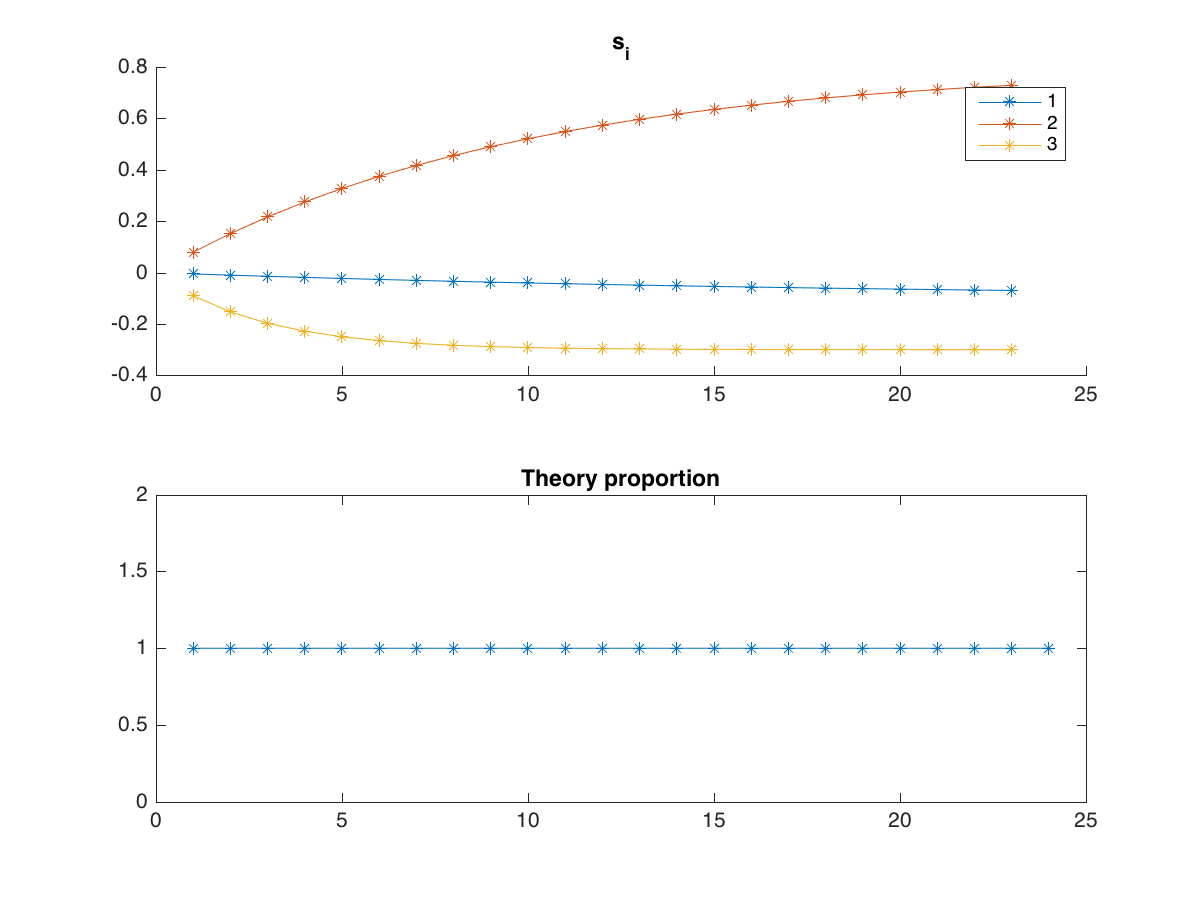
\includegraphics[width=.9\linewidth]{./img/plan2.png}
\captionof{figure}{Plan 2}
\end{center}
\begin{center}
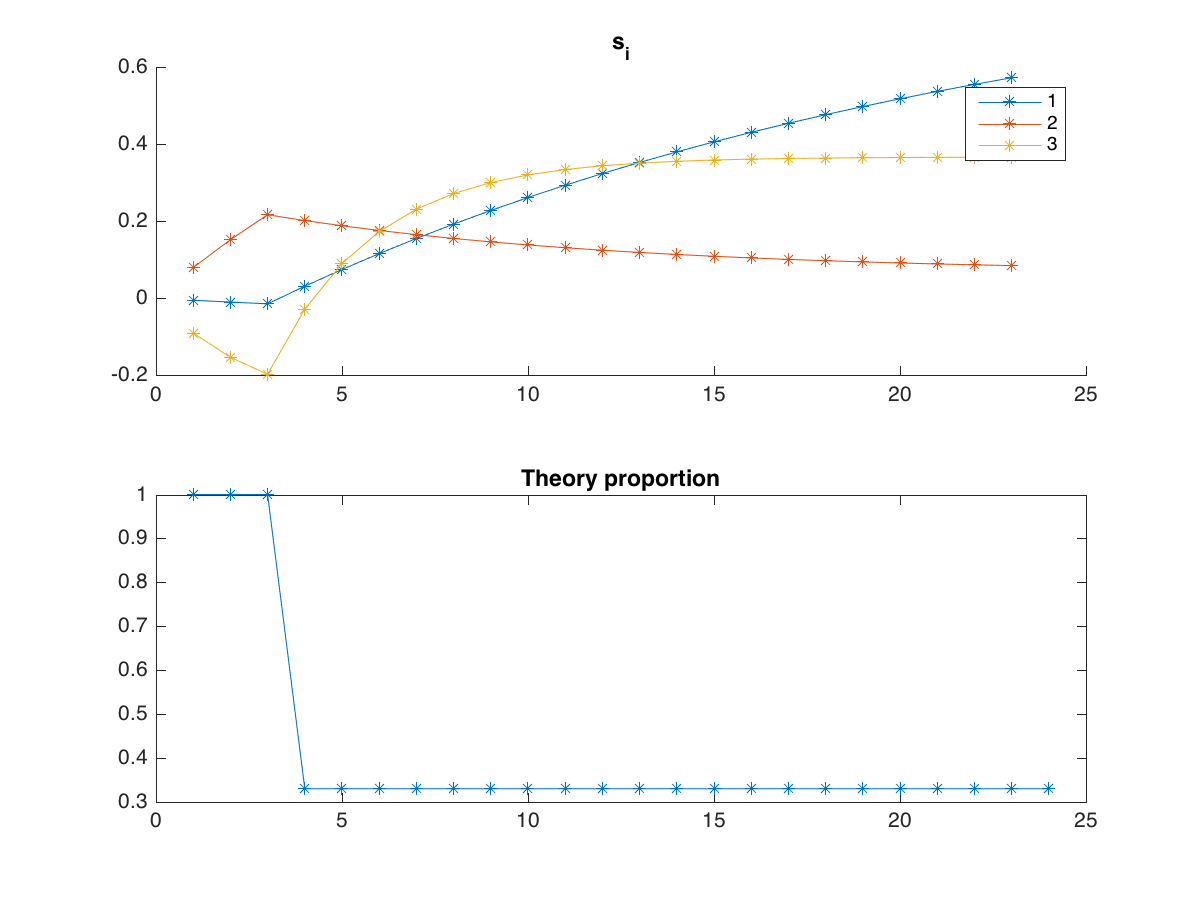
\includegraphics[width=.9\linewidth]{./img/plan3.png}
\captionof{figure}{Plan 3}
\end{center}
\begin{center}
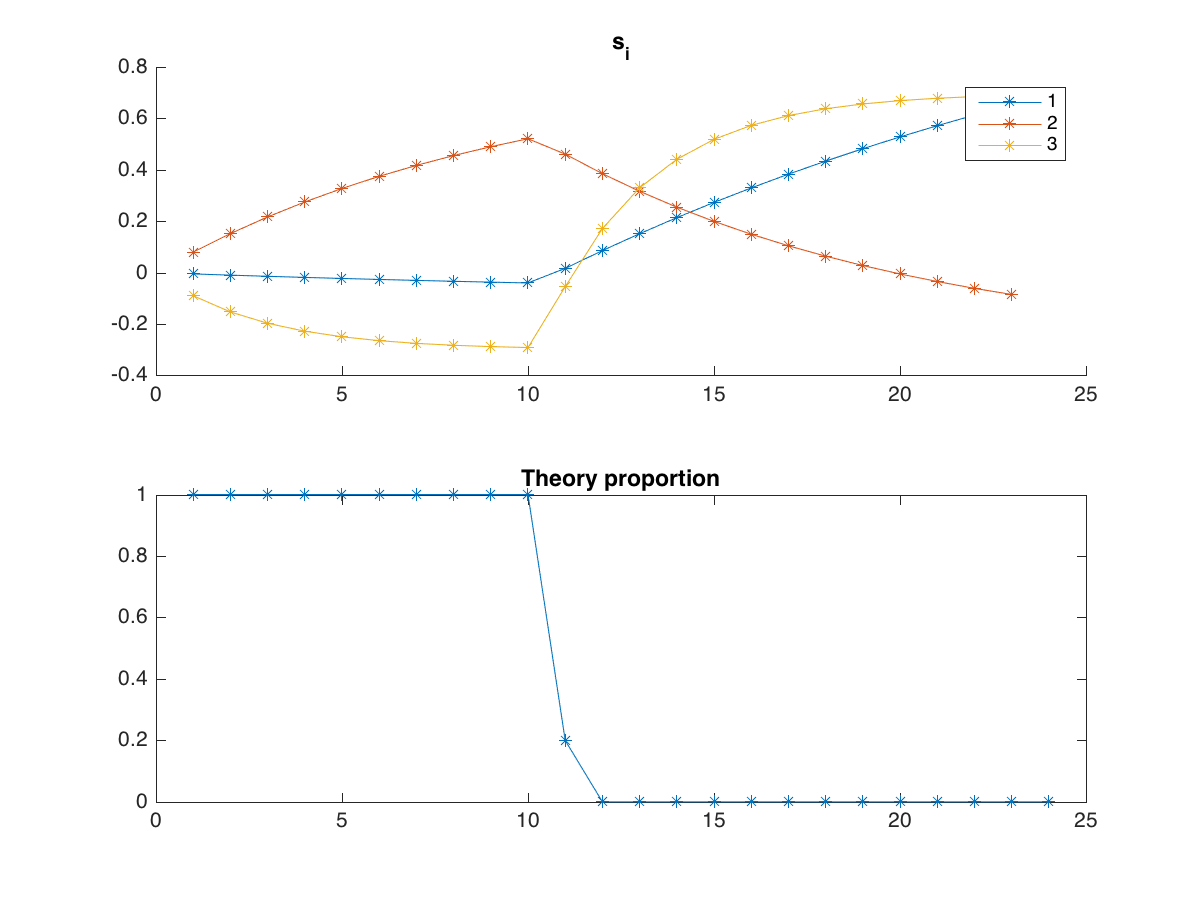
\includegraphics[width=.9\linewidth]{./img/plan4.png}
\captionof{figure}{Plan 4}
\end{center}


\section{Problem 3}
\label{sec:orgheadline4}
\(S \subseteq \mathbb R^n\).

\begin{itemize}
\item Let \(C\) a convex contating set containing \(S\), and let \(x = \sum_i \lambda_i x_i\) convex combination of element of \(S\) and thus of element of \(C\), so \(x \in C\). Therefore \(conv(S) \subset \cap_{S \subset C, C \text{ convexe}} C\)

\item The convex hull is a convexe set containing \(S\), so \(\cap_{S \subset C, C \text{ convexe}} C \subset  conv(S)\).
\end{itemize}

As a conclusion: \(conv(S) = \cap_{S \subset C, C \text{ convexe}} C\).


\section{Problem 4}
\label{sec:orgheadline5}
a)
\(\mathcal G \rightarrow \mathcal G, Q \rightarrow Q_iQ\)  is an injection because \(Q_i\) is invertible, so it is a bijection (because \(\mathcal G\) is finite), therefore:
$$Q\bar x = \frac1k \sum_{Q \in \mathcal G} Q_iQ = \frac1k \sum_{Q \in \mathcal G} Qx = \bar x$$
so \(\bar x \in \mathcal F\).

b) \(f(\bar x) \le \sum_i \frac1k f(Q_ix) = \frac1k \sum_i  f(x) = f(x)\)

c) Let \(x\) be a solution to the \(\mathcal{G}\) invariant optmization problem. Then \(\bar x \in \mathcal F\) is also a solution. Indeed:

\begin{itemize}
\item \(f_0(\bar x) \le f_0(\bar x)\)
\item for \(j\), \(f_j(x) \le 0 \implies \forall i f_j(Q_i x) \le 0 \implies  \frac1k \sum_i f_j(Q_i x) \le 0\)
\item \(f_j\) is convexe, so \(f_j(\bar x)  \le \frac1k \sum_i f_j(Q_i x) \le 0\)
\end{itemize}

Conclusion: \(f_0(\bar x) \le f_0(x)\) and \(\bar x\) is in the feasible set, which means \(\bar x\) is optimal.

d) Let \(\mathcal G\) be the set of all permutations in \(\mathbb R^{n \times n}\). It is clear that this set is a finite (of size \(n!\) ) group.

Let \(x\) be a minimizer that is stable with respect to all permutations (such \(x\) exists by the previous question), and let \(2 \le j \le n\), and \(Q\) be the matrix that permutates the 1st and jth vector of the canonical basis.
Then \(x_1 = (Px)_1 = x_j\).

Therefore \(x\)  has the form \(x_11, x_1 \in \mathbb R\).


\section{Problem 5}
\label{sec:orgheadline6}

The problem can be formulated as follow:
$$\min_{x \in S_1, y \in S_2} ||x - y||$$

\begin{minted}[frame=lines,linenos=true]{matlab}
% Input
P = [ 1 -0.6 0.2; 
      -0.6 2.6 0.6;
      0.2 0.6 0.4
    ] ;
xc = [2 2 2]';
n = 3;

% Optimization
cvx_begin
variable x(n)
variable y(n)
minimize norm(x - y)
subject to
norm(x, 1) <= 1
(y-xc)' * P * (y - xc) <= 1
cvx_end

round(horzcat(x, y), 3)
\end{minted}



The optimal value is \(1.9372\), attained for:

\begin{center}
\begin{tabular}{rr}
x & y\\
\hline
0.305 & 1.458\\
0.695 & 1.849\\
0 & 1.045\\
\end{tabular}
\end{center}



\section{Problem 6}
\label{sec:orgheadline7}
\begin{itemize}
\item \(P_2 \subseteq P_1\) ?
\begin{itemize}
\item \begin{itemize}
\item \(P_1\) facet description
\item \(P_2\) vertex description
\item \textbf{Algorithm}: Check that for each vertex \(v\) in \(P_2\) if \(v \in P_1\) (\(Av \le b\)), the result follow from the fact that \(P_2\) is the convex hull of its vertices.

\item \textbf{Complexity}: \(O(N D^2M)\) where \(D\) is the dimension, \(M\) the number of facets, and \(N\) the number of vertices.
\end{itemize}

\item \begin{itemize}
\item \(P_1\) vertex description \(y_1, \ldots, y_m\)
\item \(P_2\) vertex description \(x_1, \ldots, x_n\)
\item \textbf{Algorithm}: Check if every vertex in \(P_2\) is a convex combination of the vertices of \(P_1\): \(y_1, \ldots, y_m\). For that, check if the following LP problems are feasible for all vertex \(x\) in \(P_2\):  \(\min_{\lambda \in \mathbb{R}^D} 0\) st \(\sum \lambda_i y_i = x, \sum_i \lambda_i = 1, \lambda \ge 0\).
\item \textbf{Complexity}: \(O(N R)\) where \(R\) is the time required to solve one of the above minimization problem. (This time is polynomial in \(D\) and \(N\))
\end{itemize}

\item \begin{itemize}
\item \(P_1\) facet description \(A_1x \le b_1\)
\item \(P_2\) facet description \(A_2x \le b_2\)
\item \textbf{Algorithm}: Check if every row  \(a_i^T\) in \(A_1\), eg Check that the following problem has a non negative solution:
\(\min_{A_2x \le b} (b_1)_i - a^T x\), which is true iff \(A_2x \le b_2 \implies A_1x \le b_1\).
\item \textbf{Complexity}: \(O(M R)\) where \(R\) is the time required to solve the above minimization problem. (This time is polynomial in \(D\) and \(M\))
\end{itemize}
\end{itemize}
\end{itemize}
\end{document}